\documentclass[../main.tex]{subfiles}
\begin{document}

\section{Werkpakket 2: Prototyping}

\subsection{Prototyping V0.1 (4 maanden)}
Het doel van het prototype is om zo snel mogelijk alle afzonderlijke stappen te testen en te bewijzen dat ze werken. Het zal in een virtuele omgeving draaien, zodat er gemakkelijk kan worden geïtereerd. Portabolt zal een interface ontwikkelen waarmee extern de batterijen aangestuurd kunnen worden. Er wordt een communicatielaag gebouwd waarmee AIP de batterijen kan aansturen. Daarnaast wordt een testprotocol ontwikkeld waarmee elke afzonderlijke stap getest en gevalideerd kan worden.

\subsection{Deliverables}
\begin{enumerate}
    \item Portabolt sturingsinterface
    \item Koppeling tussen All in Power, Portabolt, Edge, Envitron
    \item Werkend prototype in een gesimuleerde omgeving
\end{enumerate}

\subsection{Urenbegroting}
Uren begroot: 1720

De sandbox wordt opgebouwd. Alles wordt in dit prototype volledig digitaal ontwikkeld om te testen of het werkt en om te zien waar we tegenaan lopen. Hiervoor worden drie modules ontwikkeld: de Price Generation Module, de Energy Profile Simulation, en de Optimization Module. In deze fase wordt nog geen daadwerkelijke data van het internet gescraped, maar alleen de werking van de modules bewezen.

\subsection{Price Generation Module}
\textbf{Objective:} Simuleer dynamische elektriciteitsprijzen die elke dag om 12:00 uur gegenereerd worden voor de volgende dag. \\
\textbf{Input:} Random variabelen die de prijzen beïnvloeden (zoals vraag, aanbod, weersomstandigheden). \\
\textbf{Output:} Een array met 24 prijzen, één voor elk uur van de volgende dag.

Bij elke run van de code wordt een array met prijzen gegenereerd. Er is een gehardcodeerde trend waarmee een normale dagelijkse prijsschommeling gesimuleerd wordt.

\begin{figure}[h!]
  \centering
  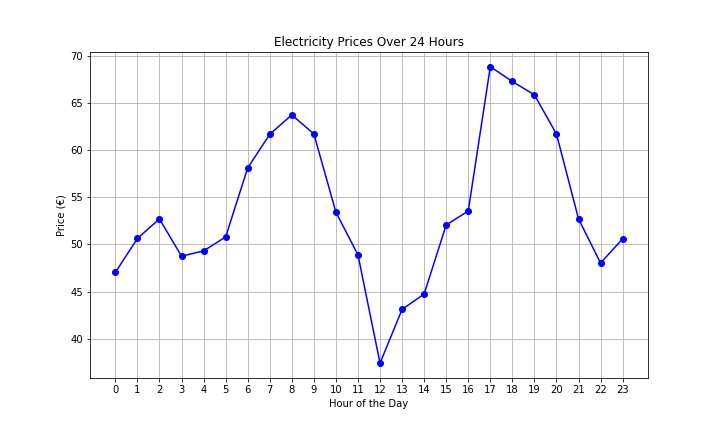
\includegraphics[width=\textwidth]{figures/price_generation_plot.png}
  \caption{Electricity Prices Over 24 Hours}
  \label{fig:price_plot}
\end{figure}

\FloatBarrier

\subsection{Energy Profile Simulation}

\textbf{Objective:} Creëer een energieverbruiksprofiel voor een gemiddeld bedrijf, dat per uur varieert. \\
\textbf{Input:} Kenmerken van het bedrijf (zoals grootte en type industrie). \\
\textbf{Output:} Een array met 24 energieverbruikswaarden, één voor elk uur van de dag.

Dit module simuleert het willekeurige energieverbruik van een bedrijf.

\subsubsection{Doel van de simulatie}
Het doel is om een representatief energieverbruikspatroon van een gemiddeld bedrijf te simuleren. Dit kan per uur, dag, week of maand worden gegenereerd. Het profiel varieert afhankelijk van het type bedrijf, werkuren, seizoensinvloeden en andere factoren.

\subsubsection{Belangrijke variabelen}
\begin{itemize}
    \item \textbf{Bedrijfsprofiel:} Werkuren, industrietype, locatie, enz.
    \item \textbf{Baseload:} Het minimum energieverbruik van het bedrijf gedurende de dag (bijv. verlichting, servers).
    \item \textbf{Piekbelasting:} Het maximale energieverbruik tijdens piekuren.
    \item \textbf{Dagelijks variërend verbruik:} Gebaseerd op het type bedrijf en de werkuren.
    \item \textbf{Seizoensgebonden variatie:} Verwarmings- of koelbehoeften.
    \item \textbf{Weekends en feestdagen:} Mogelijk lager verbruik.
\end{itemize}

\subsubsection{Simulatiemethoden}
\begin{itemize}
    \item \textbf{Random generation:} Gebruik een stochastisch model om het energieverbruik te genereren met een bepaalde spreiding rond gemiddelde waarden.
    \item \textbf{Tijdreeksanalyse:} Gebruik historische data (indien beschikbaar) om een tijdreekspatroon te simuleren.
\end{itemize}

\subsubsection{Python Code Structuur}
De code voor de simulatie wordt gestructureerd in verschillende componenten:

\paragraph{Main Simulation Script (main.py)} Dit script start de simulatie, genereert het energieprofiel en visualiseert het resultaat.
\begin{itemize}
    \item Initialiseer de simulatie.
    \item Roep de functies aan om energieverbruiksprofielen te genereren.
    \item Visualiseer de resultaten door de data te plotten.
\end{itemize}

\paragraph{Company Profile (company\_profile.py)} Dit script bevat functies om een bedrijfsprofiel te definiëren, bijvoorbeeld voor een industrieel bedrijf, kantoor of winkel.
\begin{verbatim}
def define_company_profile():
    # Return een standaard bedrijfsprofiel op basis van categorie.
\end{verbatim}

\paragraph{Energy Profile Generator (energy\_profile.py)} Dit script bevat de logica voor het genereren van energieverbruiksprofielen.
\begin{verbatim}
def generate_daily_profile(company_profile):
    # Genereert het dagelijkse energieverbruik op basis van het bedrijfsprofiel.

def apply_seasonal_variation(profile):
    # Past seizoensgebonden variaties toe op het energieverbruik.

def simulate_weekends(profile):
    # Voegt weekend- en feestdagvariaties toe.
\end{verbatim}

\paragraph{Utilities (utils.py)} Dit script bevat handige functies, zoals voor het genereren van random verbruikswaarden, het plotten van de data, enz.

\subsubsection{Simulatieverloop}
\begin{itemize}
    \item Genereer eerst een basis energieprofiel voor een gemiddelde dag.
    \item Pas vervolgens variaties toe voor piekbelasting, weekends en seizoensgebonden schommelingen.
    \item Visualiseer de resultaten met grafieken om een duidelijk overzicht van het verbruik te geven.
\end{itemize}

\subsubsection{GitHub-structuur}
Maak de volgende mappen en bestanden in de \texttt{energyprofile} folder:
\begin{verbatim}
energyprofile/
|-- main.py
|-- company_profile.py
|-- energy_profile.py
|-- utils.py
|-- data/
    |-- (eventuele historische data of configuratiebestanden)
\end{verbatim}

\subsubsection{Visualisatie}
Gebruik \texttt{matplotlib} om het energieverbruik over tijd te visualiseren.

\subsection{Optimization Module (Trading Algorithm)}
\textbf{Objective:} Ontwikkel een algoritme dat beslist wanneer elektriciteit gekocht of verkocht moet worden, gebaseerd op prijsfluctuaties en het energieverbruik van het bedrijf. \\
\textbf{Input:} Een prijsarray en een energieverbruiksarray. \\
\textbf{Output:} Een optimalisatiestrategie die maximale winst oplevert door elektriciteit te kopen op het laagste punt en te verkopen op het hoogste punt.

\end{document}
